


\section{绪论}
\subsection{XXXXXX}
\subsubsection{XXXXXX}
XXXXXXXXXXXXXXXXXXXXXXXXXXXXXXXXXXXXXXXXXXXXXXXXXXXXXXXXXXXXXXXXXXXXXXXXXXXXXXXXXXXXXXXXXXXXXXXXXXXX。

\begin{center}
    .......\\
    .......\\
    .......
\end{center}

\section{XXXXXX}

公式示例
\begin{equation}
	c_i=f(w \cdot X_{i:i+h-1} +b)
\end{equation}

代码示例\footnote{这是脚注}
\begin{minted}[
	frame=lines,
	framesep=2mm,
	baselinestretch=1.2,
	fontsize=\footnotesize,
	linenos
]{python}

import numpy as np

def incmatrix(genl1,genl2):
    m = len(genl1)
    n = len(genl2)
    M = None #to become the incidence matrix
    VT = np.zeros((n*m,1), int)  #dummy variable

    #compute the bitwise xor matrix
    M1 = bitxormatrix(genl1)
    M2 = np.triu(bitxormatrix(genl2),1)

    for i in range(m-1):
        for j in range(i+1, m):
            [r,c] = np.where(M2 == M1[i,j])
            for k in range(len(r)):
                VT[(i)*n + r[k]] = 1;
                VT[(i)*n + c[k]] = 1;
                VT[(j)*n + r[k]] = 1;
                VT[(j)*n + c[k]] = 1;

                if M is None:
                    M = np.copy(VT)
                else:
                    M = np.concatenate((M, VT), 1)

                VT = np.zeros((n*m,1), int)

    return M
\end{minted}


图示例
\begin{figure}[!htb]
	\centering
	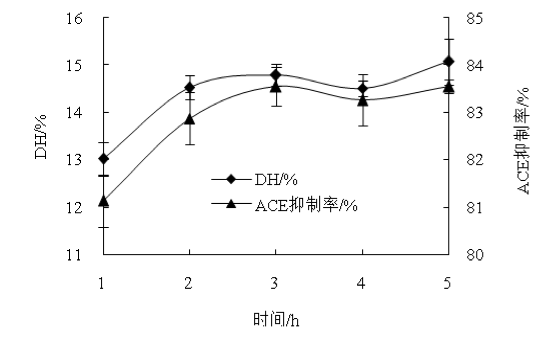
\includegraphics{images/example_figure1.png}
	\caption{酶解时间对DH与ACE抑制率的影响}
\end{figure}

\begin{figure}[!htb]
	\centering
	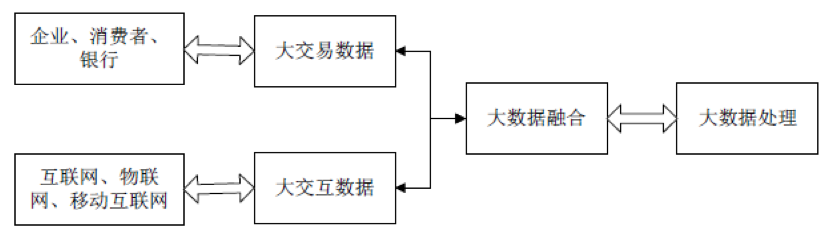
\includegraphics{images/example_figure2.png}
	\caption{XXXXXXXXXX}
\end{figure}

\clearpage
表示例
\begin{table}[!htb]
\centering
\caption{三种肌球蛋白/多糖混合凝胶的红外光谱数据}
\begin{tabular}{lcccc}
\hline
Treatment           & \multicolumn{4}{c}{FT-IR spectra numbers (cm$^{−1}$)} \\ \cline{2-5} 
                    & PK1        & PK2        & PK3        & PK4       \\ \hline
Myosin gel          & 3439       & —          & 1655       & 1106      \\
Myosin+ 1\% KCG gel & 3358       & 3006       & 1655       & 1131      \\
Myosin+ 1\% LBG gel & 3366       & 3006       & 1655       & 1106      \\
Myosin+ 1\% WSC gel & 3439       & —          & 1655       & 1106      \\ \hline
\end{tabular}
\end{table}

\begin{table}[!htb]
\centering
\caption{分栏表}
\begin{tabular}{ccccc}
\hline
年度                    & 产品  & 产量    & 销量    & 产值  \\ \hline
\multirow{2}{*}{2004} & 手机  & 11000 & 10000 & 500 \\
                      & 计算机 & 1100  & 1000  & 280 \\ \hline
\multirow{2}{*}{2005} & 手机  & 16000 & 13000 & 550 \\
                      & 计算机 & 2100  & 1500  & 320 \\ \hline
\end{tabular}
\end{table}





\begin{table}[!htb]
    \centering
    \caption{三种肌球蛋白/多糖混合凝胶的红外光谱数据}
    \begin{tabular}{lcccc}
        \hline
        Treatment           & \multicolumn{4}{c}{FT-IR spectra numbers (cm$^{−1}$)} \\ \cline{2-5} 
                            & PK1        & PK2        & PK3        & PK4       \\ \hline
        Myosin gel          & 3439       & —          & 1655       & 1106      \\
        Myosin+ 1\% KCG gel & 3358       & 3006       & 1655       & 1131      \\
        Myosin+ 1\% LBG gel & 3366       & 3006       & 1655       & 1106      \\
        Myosin+ 1\% WSC gel & 3439       & —          & 1655       & 1106      \\ \hline
    \end{tabular}
\end{table}